\documentclass[a4]{article}
\usepackage[czech]{babel}
\usepackage[utf8]{inputenc}
\usepackage{graphicx}
\graphicspath{ {images/} }
%\usepackage{a4wide}
\usepackage[top=2.5cm, bottom=2.5cm, left=4cm, right=2.5cm]{geometry}
\usepackage{wrapfig}
\usepackage{url}
\usepackage{amsmath,amsfonts,amssymb,amsthm}
\usepackage{subcaption}

\begin{document}

\title{Blekota --- generování zvuku pomocí rekurentních neuronových sítí}
\author{Václav Volhejn}

\begin{titlepage}
\centering
{\scshape\Large Gymnázium Jana Keplera \par}
{Obor vzdělání: Gymnázium 79-41-K/81 \par}
\vspace{1.5cm}
{\huge\bfseries Blekota --- generování zvuku pomocí rekurentních neuronových sítí \par}
\vspace{2cm}
{\Large\itshape Václav Volhejn \par}
\vfill
Vedoucí práce: \par
Tomáš \textsc{Obdržálek}
\vfill
{\large Praha, 2017} %\today
\end{titlepage}

\tableofcontents
\section{Anotace}
Blekota používá rekurentní neuronové sítě aby předpověděl, jak bude pokračovat zadaný trénovací zvuk na základě jeho dosavadních hodnot. Generujeme nový zvuk tak, že necháme Blekotu předpovědět pokračovaní zvuku a tuto předpověď ke zvuku přidáme a proces opakujeme. Zkoumáme účinnost tohoto modelu při předvídání a vytváření lidského hlasu a vliv hyperparametrů na kvalitu předpovědí.
\noindent\rule[0.5ex]{\linewidth}{0.8pt}
Blekota uses recurrent neural networks to predict how a given training sound continues based on the sound's previous data. We generate new sounds by letting Blekota predict the continuation of a sound, append the prediction to the sound and repeat the process. We analyse the model's efficiency when predicting and creating human speech and the influence of hyperparameters on the predictions' quality.
\section{Prohlášení}
Prohlašuji, že jsem jediným autorem této maturitní práce a všechny citace, použitá literatura a další zdroje jsou v práci uvedené. Tímto dle zákona 121/2000 Sb. (tzv. Autorský zákon) ve znění pozdějších předpisů uděluji bezúplatně škole Gymnázium Jana Keplera, Praha 6, Parléřova 2 oprávnění k výkonu práva na rozmnožování díla (§ 13) a práva na sdělování díla veřejnosti (§ 18) na dobu časově neomezenou a bez omezení územního rozsahu.

\vfill

\section{Úvod}
Projekt byl inspirován článkem \textit{The Unreasonable Effectiveness of Recurrent Neural Networks} \cite{unreasonable}. Karpathy v něm využívá rekurentní neuronové sítě (RNN) ke generování textu, který se podobá nějakému vzorovému; model se například naučil psát Shakespearovské hry či články na Wikipedii. Blekota se snaží tyto výsledky reprodukovat ve sféře zvuku, tj. generovat zvuky, které mají znít podobně, jako ten, na kterém se model učí.

Zvuk je kvůli hustotě dat větší výzva, než text --- aby model generující text vytvořil smysluplnou větu, musí (dostatečně) správně předpovědět desítky znaků. Oproti tomu jedna sekunda zvuku odpovídá tisícům vzorků --- CD například používá vzorkovací frekvenci 44,1 kHz. Zvukový model proto musí pracovat na výrazně větší časové škále, aby dával srovnatelné výsledky.

\begin{figure}[h]
\centering
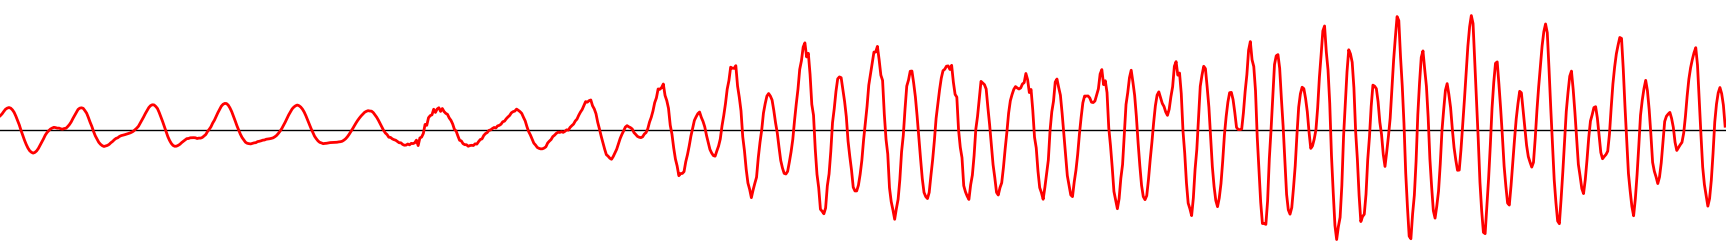
\includegraphics[width=\textwidth]{voice_example}
\caption{Graf 1000 vzorků zvuku o vzorkovací frekvenci 8 kHz. Zvuk odpovídá hlásce \textit{j}.}
\end{figure}

\subsection{Rekurentní neuronové sítě}
Cílem \textit{supervised learning} (\uv{učení s učitelem}) je naučit výpočetní model (např. neuronovou síť) přiřazovat k daným vstupům správné výstupy na základě označených dat, tj. dat, kde je k dispozici vždy dvojice vstup---správný výstup.

Například bychom mohli chtít model naučit rozpoznávat, zda je na zadaném obrázku kočka. K trénovaní bychom modelu dali milion obrázků, o kterých bychom věděli, zda je na nich kočka, nebo ne. Model vždy zadaný obrázek nějak zanalyzuje a jako výstup dá pravděpodobnost, že je na obrázku kočka. Protože víme, jaká je správná odpověď, dokážeme upravit parametry modelu (čisla, které určují jeho chování) tak, aby na tento konkrétní vstup dával trochu lepší odpověď --- pokud byla na obrázku kočka, poučený model by jako výstup nyní dal vyšší pravděpodobnost, a naopak.

Po našem modelu chceme, aby na základě dosavadního zvukového signálu předpověděl jeho další kousek (správně vzorek; \textit{sample}). Zde se tradiční postupy nehodí --- normální neuronové sítě nemají žádný stav, nepracují s konceptem minulosti. To, jestli byla na minulém obrázku kočka, nemá vliv na to, jestli bude na příštím. V tomto případě ale další vzorek na minulých zjevně závisí.

Tento problém řeší model zvaný rekurentní neuronová síť (\textit{Recurrent Neural Network}, RNN). Na první pohled funguje model podobně jako běžné modely --- dostane nějaký vstup a dá nějaký výstup. Když ale dostane vstup, změní nějak svůj vnitřní stav, takže každý výstup je ovlivňen všemi vstupy, které přišly před ním.

\section{Teorie} \label{teorie}

Formálně máme vektor $x$, ve kterém $x_t$ je hodnota $t$-tého vzorku napodobovaného zvuku. Po našem modelu chceme, aby předpověděl $x_{t+1}$ z předchozích $t$ vzorků, tj. aby určil $p(x_{t+1} | x_{1} \dots x_{t})$.

Přesněji, model má jako vstup $x_t$ (další vzorek zvuku z trénovacího souboru) a jako výstup přiřazuje každé z možných hodnot $a$ pravděpodobnost, se kterou si myslí, že bude následovat, tj. pravděpodobnost, že $x_{t+1}=a$.

Ve zvukových souborech se vzorky obvykle ukládají jako 16-bitová čísla, takže bychom museli v každém kroku spočítat $2^{16} = 65 536$ pravděpodobností. Pro zjednodušení kvantujeme vzorky na 256 možných hodnot stejným způsobem, jako WaveNet od Googlu \cite{wavenet}. Jedná se o $\mu$-\textit{law compander} (ITU-T, 1988) \cite{mulaw}, který hodnoty nelineárně transformuje tak, že přesněji zachová vzorky blíže nule, kde jsou nuance důležitější.

Abychom dále redukovali množství dat, učíme model na zvucích s vzorkovací frekvencí 8 kHz. Následkem toho se ale zvuk už výrazně zkresluje, protože maximální frekvence zaznamenatelná signálem s frekvencí $f_s$ je $\frac{f_s}{2}$ (Nyquistova frekvence), takže se ztrácí složky s frekvencí nad 4 kHz.

Rekurentní neuronová síť má stav $h$, což je vektor reálných čísel od -1 do 1. Jeden krok sítě obnáší výpočet nového stavu $h_t$ z předchozího stavu $h_{t-1}$ a vstupu pro tento krok $x_t$. $x_t$ je nejnovější vzorek zvuku, jehož další vzorek chceme předvídat (model se tedy snaží odhadnout, jaká bude hodnota $x_{t+1}$).

Nabízí se $x$ reprezentovat jako jediné číslo, které by odpovídalo hodnotě vzorku (kterou jsme kvantovali na 256 hodnot, viz výše). Mocnější reprezentace ale docílíme \textit{one-hot encoding}; vstup bude vektor o 256 prvcích, které odpovídají jednotlivým možným hodnotám vzorků. V každém $x$ budou všechny hodnoty 0, kromě hodnoty toho prvku, který odpovídá hodnotě momentálního vzorku --- ten nastavíme na 1.

\subsection{Gated Recurrent Unit}

Blekota používá variantu RNN zvanou \textit{Gated Recurrent Unit} (GRU), kterou uvedli Cho et al. (2014) \cite{gru}. Výpočet $h_t$ v ní vypadá takto:

\begin{align*}
r_t &= \sigma(W_r \cdot [x_t, h_{t-1}]) \\
h'_t &= tanh(W \cdot [x_t, r_t * h_{t-1}]) \\
z_t &= \sigma(W_z \cdot [x_t, h_{t-1}]) \\
h_t &= (1 - z_t) * h_{t-1} + h'_t * z_t
\end{align*}

kde $[a, b]$ je skládání vektorů za sebe (z vektorů o rozměrech $[N,1]$ a $[M,1]$ vytvoříme jeden o $[N+M,1]$ vektor), $\cdot$ znamená maticové násobení (v našem případě jen násobení matice-vektor); ostatní aritmetické operace jsou aplikovány po složkách. $\sigma$ je logistický sigmoid
% definovaný jako $$\sigma(x) = \frac{1}{1 + e^{-x}}$$    % je potřeba?
který svůj vstup "zmáčkne" do intervalu $(0, 1)$. Hyperbolický tangens hraje podobnou roli, ale jeho obor hodnot je $(-1, 1)$. $W$, $W_r$ a $W_z$ jsou matice, které tvoří parametry modelu a při trénování jejich hodnoty optimalizujeme. Proberme význam jednotlivých kroků výpočtu:

$r_t$ je \textit{reset gate}, který vypočítáme z momentálního vstupu a předchozího stavu. Rozhoduje, co z předchozího stavu model zapomene při výpočtu nového - když jsou jeho hodnoty blízko 0, při výpočtu $h'_t$ nezáleží už tolik na $h_{t-1}$ a model musí počítat zejména s $x_t$; může tak zapomenout hodnoty předchozího stavu, které jsou nyní nepotřebné.

$h'_t$ je \textit{kandidát} (na nový stav), který počítáme z $x_t$ a částečně zapomenutého $h_{t-1}$. Po vynásobením maticí $W$ výstup necháme projít přes $tanh$, aby zůstaly hodnoty $h_t$ v intervalu $(-1, 1)$.

Samotný $h_t$ pak spočítáme váženým průměrem mezi $h'_t$ a $h_{t-1}$. Váhy určuje $z_t$ --- pokud je nějaká hodnota $z_t$ blízko 0, bude $h_t$ v tomto podobná, jako předtím (tj. bude si dál pamatovat původní hodnotu $h_{t_1}$), naopak pokud bude blízko 1, hodnota $h_t$ v tomto prvku bude takřka nahrazena novou. GRU se tak může rozhodnout, kdy co zapomenout.

Poznamenávám, že zde ve výpočtu pro přehlednost vynechávám \textit{bias} --- ve skutečnosti je u každého maticového násobení k násobenému vektoru přidána konstantní 1, takže např. výpočet $r_t$ vypadá takto: $r_t = \sigma(W_r \cdot [x_t, h_{t-1}, 1])$. Tato konstanta umožňuje modelu při násobení ke každé hodnotě přičíst nějakou konstantu (závislou v tomto případě na nějakém prvku $W_r$).

\subsection{Výstup}
Samotné $h_t$ nám ale nestačí, je jen nějaký vnitřní stav modelu. Chceme přeci předvídat hodnotu $x_{t+1}$. Proto ještě musíme zadefinovat $y_t$ a $p_t$:

\begin{align*}
y_t &= W_y \cdot h_t \\
p_t &= \frac{e^{y_t}}{\sum e^{y_t}}
\end{align*}

$y_t$ je vektor o 256 prvcích, které znamenají váhy jednotlivých možných hodnot $x_{t+1}$: čím vyšší hodnota prvku, tím vyšší je podle modelu pravděpodobnost, že $x_{t+1}$ bude právě tento prvek. V $p_t$ pak z vah tvoříme skutečné pravděpodobnosti pomocí \textit{softmax funkce}, která vyšší váze přiřadí vyšší pravděpodobnost a zařídí, že prvky $p_t$ se sečtou na 1.

%\subsubsection{Generování}

\begin{figure}[h]
\centering
\begin{subfigure}{.5\textwidth}
\centering
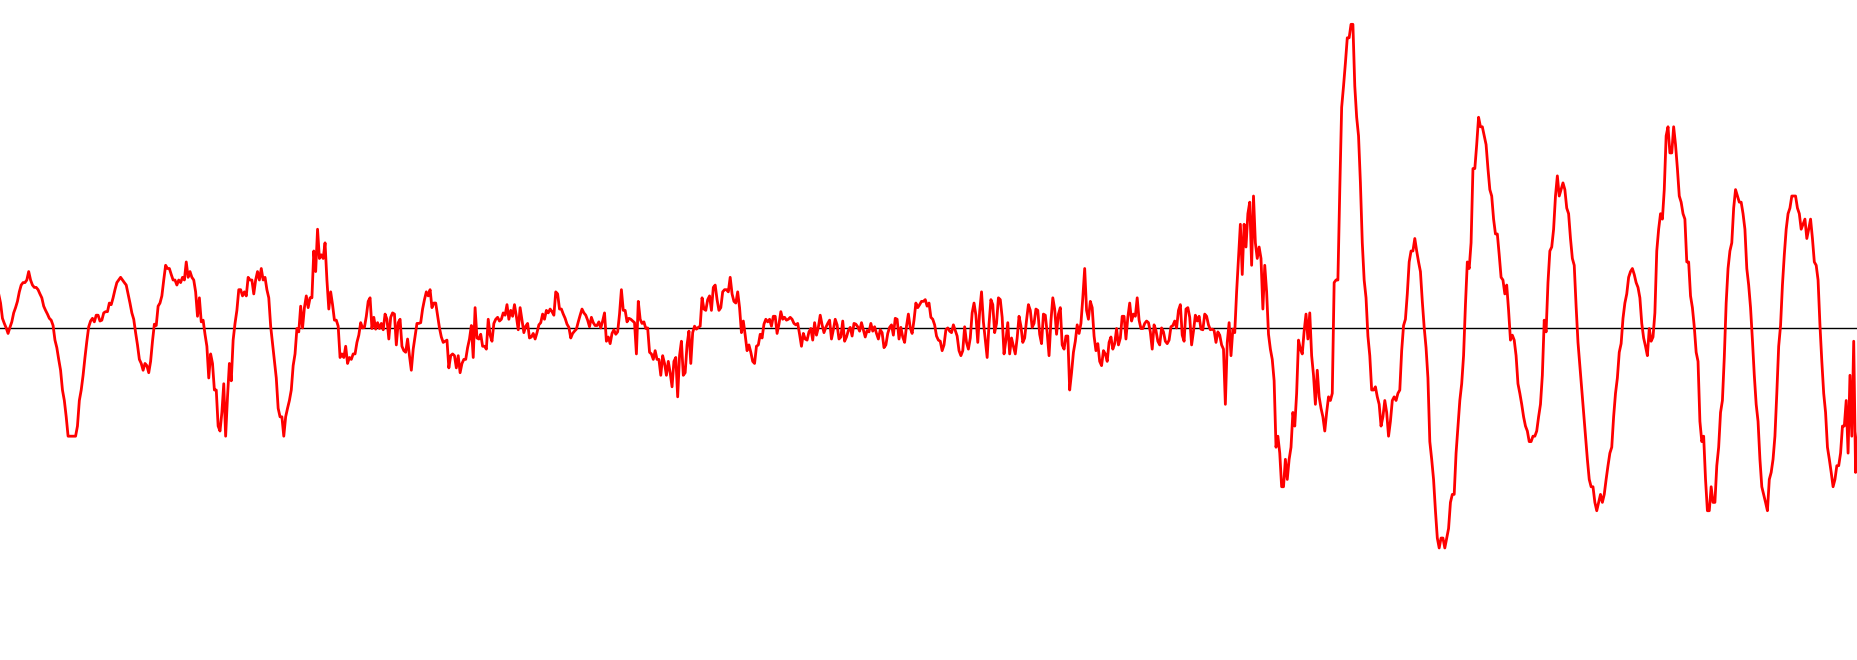
\includegraphics[width=0.9\linewidth]{waveform_1}
\end{subfigure}%
\begin{subfigure}{.5\textwidth}
\centering
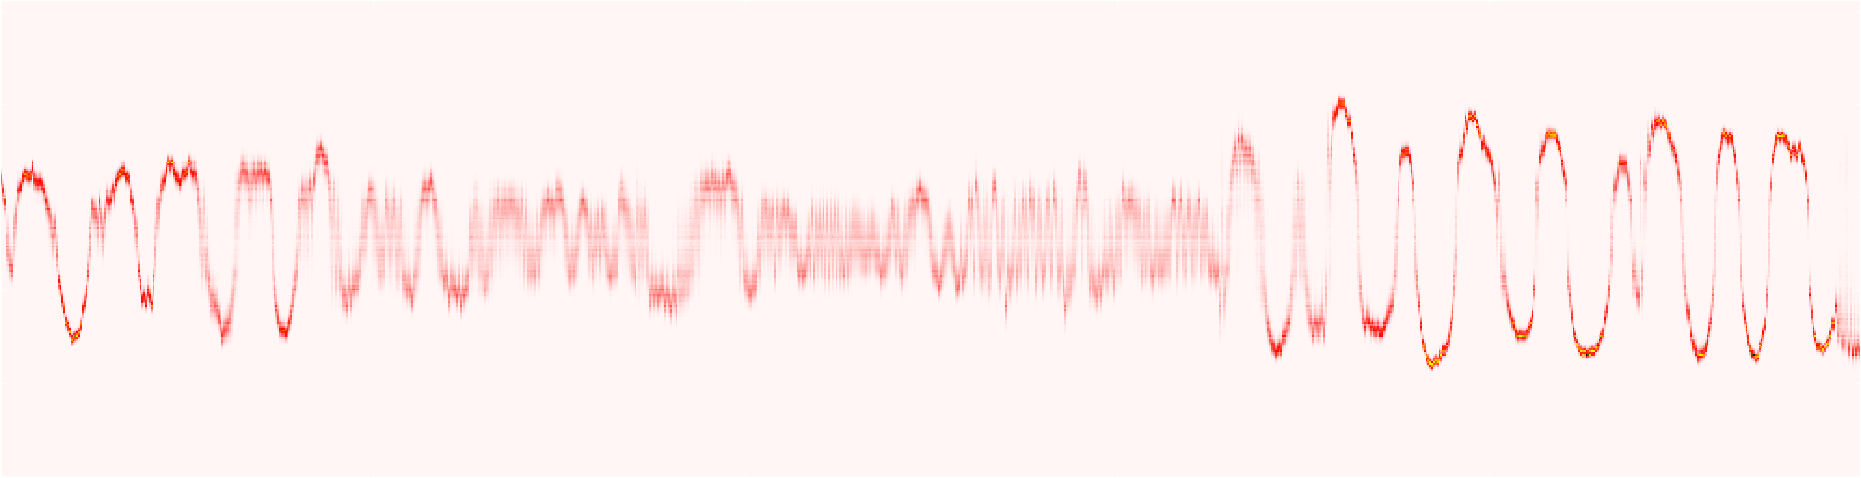
\includegraphics[width=0.9\linewidth]{heatmap_1_v2}
\end{subfigure}
\caption{Ukázka 1000 vzorků (0,125 s) vygenerovanému zvuku a teplotní mapa jemu odpovídající. Hodnoty vzorků, které model považuje za pravděpodobnější, jsou tmavší. Rozmazaná místa pak odpovídají nejistotě, kde model považuje více různých hodnot za podobně pravděpodobné. \protect \footnotemark}
\end{figure}

\footnotetext{Důvod, proč tvar Obr. \ref{waveform_1} nevypadá stejně jako Obr. \ref{heatmap_1} je ten, že v teplotní mapě má každá hodnota shodnou výšku; jedná se o obrázek s výškou 256 pixelů. Oproti tomu v praxi jsou hodnoty kvantované nelineárně; viz sekce \ref{teorie} Teorie. Ve výsledku to znamená, že teplotní mapa je oproti skutečnosti kolem prostředka vertikálně protažená.}

Jak ale pomocí tohoto modelu generovat nový zvuk, ne pouze předvídat vzorky existujícího? Při trénování je postup takový, že napřed dáme modelu jako vstup $x_1$, ten nám jako výstup dá pravděpodobnosti různých hodnot $x_2$. Pak mu dáme jako vstup $x_2$ a on předpoví $x_3$, atd.

Zde ale žádné $x$ neznáme. To vyřešíme tak, že hodnotu prvního vstupu, tj. $x_1$ zvolíme arbitrárně. Model pak vytvoří nějakou pravděpodobnostní distribuci hodnot $x_2$. Podle této distribuce vybereme jednu z hodnot a prohlásíme ji za skutečné $x_2$. Tuto hodnotu pak modelu dáme jako další vstup. Toto můžeme opakovat, jak dlouho chceme. Výsledné $x$ je pak vygenerovaný zvuk.

\subsection{Učení}
Abychom model mohli učit, potřebujeme nějak ohodnotit, jak dobré předpovědi dělá. Používáme \textit{cross-entropy loss} --- pro naše účely stačí, že cena (chyba) nějaké předpovědi je $-\log(p_{i})$, kde $p$ je pravděpodobnostní distribuce, kterou model vytvořil, a $i$ je index skutečné hodnoty dalšího vzorku. Čím nižší pravděpodobnost model přiřadí správné hodnotě, tím větší cena.

\begin{wrapfigure}{r}{0.5\textwidth}
    \centering
    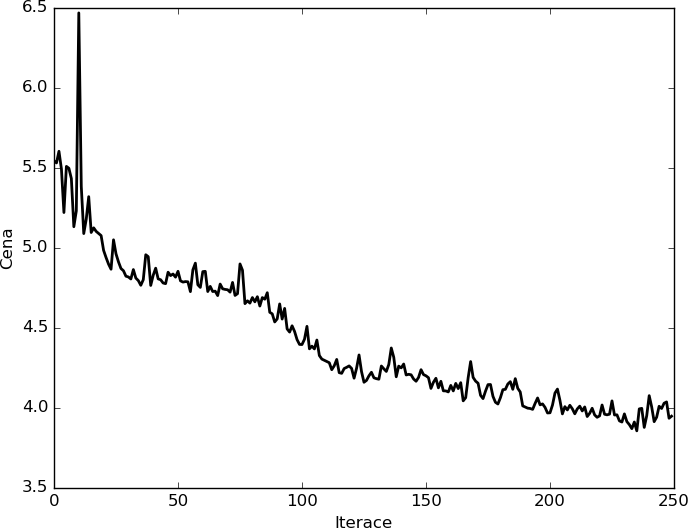
\includegraphics[width=0.5\textwidth]{loss_4}
    \caption{Graf ceny podle počtu iterací}
\end{wrapfigure}

Podstatnější než sama hodnota ceny je ale její gradient. Model učíme pomocí \textit{gradient descent}. Všechny kroky výpočtu jsou diferenciovatelné, takže můžeme spočítat gradient (parciální derivace) všech proměnných --- jinak řečeno, dozvíme se, jakým směrem musíme posunout parametry modelu ($W_y$, $W$, $W_r$, $W_z$), aby se cena snížila.

Trénování pak vypadá tak, že necháme model předvídat určitou část zvuku (kolem 100 vzorků), pak spočítáme gradient a změníme parametry podle gradientu. Opakováním tohoto procesu model postupně zlepšuje své předpovědi. Ke konvergenci potřebuje zpravidla tisíce iterací (v posledních pokusech jsem pracoval s 10000 iteracemi).

Přesně jakým způsobem měníme parametry závisí na použité optimalizační metodě. Starší verze Blekoty používaly AdaGrad \cite{adagrad}, nyní používá RMSProp \cite{rmsprop}, který se ukázal být výrazně účinnější. Při vytváření programu jsem také dlouho bojoval s laděním rychlosti učení (\textit{learning rate}) $\alpha$, která říká, jak moc chceme v každé změně parametry upravit. Příliš velké $\alpha$ může optimální hodnoty \uv{přestřelit}, když parametry změní moc.

\subsection{Vrstvení}
Mocná technika, která se objevuje napříč strojovým učením, je použití více \textit{vrstev} (layers). Můžeme udělat to, že vezmeme výstup jednoho GRU a dáme ho jako vstup dalšího. Takto můžeme napojit libovolně mnoho GRU za sebe. Každé z nich vstup nějakým způsobem zpracuje a přiblíží se cílovému výstupu -- předpovědím.

Místo základního schématu \textit{vstup (zvuk) $\rightarrow$ GRU $\rightarrow$ výstup (předpověď)} tak můžeme dostat pomocí tří GRU toto: \textit{vstup (zvuk) $\rightarrow$ GRU $\rightarrow$ GRU $\rightarrow$ GRU $\rightarrow$ výstup (předpověď)}. Vícevrstvé modely opravdu pracují mnohem lépe, než jednovrstvé -- důvodem by mohlo být, že vrstvy blíže u výstupu pracují na dlouhodobější úrovni, protože jejich vstup je stav předchozí vrstvy, který se mění pomaleji, než původní zvukový vstup. Všechny aspoň obstojné výsledky z této práce používají vícevrstvé GRU. V kódu nazývám jednu vrstvu \textit{GRULayer} a celou síť dohromady jednoduše \textit{GRU}.

\section{Výsledky}
\begin{center}
\begin{tabular}{ |c|c|c|c|c|c|c|c|c| }
\hline
Název 					& Popis 									&$h_n$&$l_n$&$t_n$&$b_n$& it & Parametry\\ \hline \hline
\verb|warble| 			& Sinusoida s oscilující frekvencí 		& 100 & 1 & 100 & 1  & 20000 &   132 956 \\ \hline
\verb|drip| 			& Pravidelně kapající voda 					& 100 & 2 & 100 & 80 & 10000 &   193 256 \\
\						& Varianta s vyšším $h_n$ 					& 256 & 2 & 100 & 80 & 10000 &   853 760 \\ \hline
\verb|hunger_artist|	& Mužský hlas; mluvené slovo v angličtině 	& 256 & 2 & 100 & 80 & 7000  &   853 760 \\
						& Varianta se třemi vrstvami ($l_n=3$) 	& 256 & 3 & 100 & 80 & 4500  & 1 247 744 \\ \hline
\verb|alice| 			& Ženský hlas; mluvené slovo v němčině 	& 256 & 3 & 100 & 80 & 9000  & 1 247 744 \\ \hline
\verb|pi| 				& Mužský hlas; číslice $\pi$ 				& 512 & 3 & 80  & 60 & 5000  & 4 461 312 \\
						& Varianta se čtyřmi vrstvami				& 300 & 4 & 80  & 60 & 13000 & 2 201 056 \\ \hline
\verb|vali| 			& Ženský hlas; mluvené slovo v češtině 	& 256 & 5 & 80  & 60 & 10000 & 2 035 712 \\ 
						& Varianta se vzorkovací frekvencí 16 kHz 	& 256 & 5 & 80  & 60 & 10000 & 2 035 712 \\ \hline
\verb|bety| 			& Ženský hlas; zpěv (slabika \uv{ma}) 		& 256 & 5 & 80  & 80 & 8000  & 2 035 712 \\ \hline
\end{tabular}
\end{center}

\textit{$h_n$ --- velikost stavového vektoru každé vrstvy; $l_n$ --- počet vrstev; $t_n$ --- délka \textit{sekvence} (kolik kroků provést před aktualizací parametrů); $b_n$ --- kolik sekvencí počítat současně; it --- počet iterací trénování; Parametry --- celkový počet parametrů modelu}
\subsection{Warble}
Zpočátku jsem hledal co možná nejjednodušší zvuky na testování modelu. Sinusoida s konstantní frekvencí byla ale příliš jednoduchá (modelu stačí předpovědět stejnou hodnotu, jako byla před periodou vlny). Použil jsem proto sinusoidu s rychle kolísající frekvencí. Použitý model byl velmi jednoduchý, ale zvuk napodobil poměrně věrně. Problém má se správným kolísáním; jeho paměť zřejmě není dostatečně dlouhodobá, aby si tyto souvislosti uvědomil.

\subsection{Drip}
Dalším krokem měl být zvuk ne uměle vytvořený, ale přirozený. Takový zvuk je mnohem méně pravidelný a proto těžší na napodobení. Chtěl jsem proto napřed použít nějaký pravidelný, jednoduchý zvuk. Dobře posloužilo pravidelné kapání vody z kohoutku. Porovnal jsem dvě varianty, z nichž jedna měla vyšší $h_n$. Ukázka zvuku první varianty ($h_n=100$) se nacházi v \verb|drip_v1.wav|, druhá pak v \verb|drip_v2.wav|. Obě už dokážou generovat nestejnorodý zvuk, který začíná jinak, než končí (narozdíl od předchozí sinusoidy, kde je zvuk \uv{spojitý}). U druhé varianty je napodobení výrazně přesnější; má také asi čtyřikrát více parametrů.

\textit{V této fázi jsem zprovoznil ukládání vytrénovaných modelů do souboru, proto nejsou starší modely dostupné k vyzkoušení.}
\subsection{Hunger Artist}
Přesunul jsem se k lidskému hlasu, který jsem pak zkoumal až do konce. Začal jsem s největší výzvou: čtený text. Zvuk je silně nepravidelný a pro model je těžké posunout se dál než k samému zvuku hlasu mluvčího, případně odlišení samohlásek. Jako trénovací soubor jsem použil povídku Franze Kafky \textit{The Hunger Artist} přečtenou Hanifem Kureishi. % http://www.openculture.com/freeaudiobooks -> gdn.book.121221.tm.Franz-Kafka-story-Hanif-Kureishi
Porovnal jsem dva modely, které se lišily jen počtem vrstev (\verb|v1| --- dvě vrstvy; \verb|v2| --- tři vrstvy). Oba modely jsem trénoval stejnou dobu z hlediska skutečného času, proto prošla \verb|v2| menším počtem iterací. Výsledky jsou ale ve \verb|v2| výrazně lepší. \verb|v1| zůstává na úrovni jednolitého šumu nebo mumlání. Oproti tomu \verb|v2| už dělá pauzy v řeči a používá různé hlásky, přestože se většinou drží zvuku anglického \textit{w}.

Zde jsem také zkoušel generovat s různou \textit{teplotou}. Všechny váhy v pravděpodobnostní distribuci umocníme na $\frac{1}{\tau}$, kde $\tau$ je teplota. Pokud $\tau<1$, budeme častěji vybírat možnosti, které model považuje za pravděpodobnější. Dostaneme často správnější, ale méně různorodé výsledky. Oproti tomu pokud $\tau > 1$, pravděpodobnosti se vyrovnávají.

U modelu \verb|v2| byla nejlepší teplota kolem 0,9. Model dělá pauzy v řeči, náznaky v intonaci a hlas zní nejpřirozeněji. Nižší teplota generuje většinou jen ticho (protože pro model je většinou nejpravděpodobnější možnost pokračovat v tichu). Naopak při vyšší teplotě nedělá pauzy vůbec a hlas zní zkresleněji, protože se model méně drží správného tvaru zvukové křivky.

\subsection{Alice}
Stejný model jako \verb|v2| u předchozího pokusu jsem aplikoval na \textit{Alices Abenteuer im Wunderland} Lewise Carrolla. Vybral jsem kapitoly 6 a 8 přečtené \textbf{KÝM}? Cílem bylo srovnat zaprvé mužský a ženský hlas a zadruhé dva různé jazyky. Bohužel tento model dával výrazně horší výsledky než předchozí; generuje většinou ticho protkané občasnými náznaky řeči. Ani při vyšší teplotě nejsou výsledky o moc lepší. Uvádím ještě ukázky z verze modelu po 7300 iteracích, která se naopak vždy dlouho drží na jedné hlásce a pauzy nedělá vůbec.
% https://librivox.org/alices-abenteuer-im-wunderland-von-lewis-carroll/ (part 6; part 8)

\subsection{Pi}
Po neúspěchu \textit{alice} jsem zvolil výrazně pravidelnější zvuk i silnější modely. Přečetl jsem za dvacet minut necelých 2000 cifer $pi$ a na tomto zvuku trénoval dva modely. \verb|v1| má velké $h_n$, ale \verb|v2| má o vrstvu více. Oba modely jsem trénoval stejnou dobu a protože \verb|v1| má asi dvakrát víc parametrů a trénuje se pomaleji, prošel méně iteracemi. Oba modely už ale stagnovaly a dále se nezlepšovaly.

\verb|v1| většinou mění mezi hláskami \textit{š} a \textit{n}. Občas slyšíme náznak čísla (typicky \textit{devět}), ale rychle se vrátí k držení jedné hlásky.
Překvapivě lepší výsledky dával \verb|v2|, který je co do počtu parametrů dvakrát menší. Dělá pauzy a co je hlavní, dokáže vyslovit jednotlivá čísla. To je opravdu složité, protože jsou velmi často dvojslabičná a poskládat za sebe všechny hlásky slova \textit{jedna} je nelehký úkol. Stává se také, že model v půlce slova zapomene, co předcházelo, a vzniknou výroky typu \textit{šenda}, což je hybrid \textit{šest} a \textit{jedna}. Přesto je působivé, že model (relativně) správně rozlišuje mezi deseti možnými slovy.
Při vyšší teplotě sklouzává stejně jako \verb|v1| k \textit{š}, možná proto, že to je hláska nejpodobnější šumu (který vzniká, když generujeme zcela náhodně).

\subsection{Vali}
Doufal jsem, že se silnějším modelem bude trénování na přirozené lidské řeči úspěšnější než v předchozích dvou případech. Nechal jsem Valerii Plevovou přečíst úryvek z \textit{1984} George Orwella. V tomto případě jsem srovnával dvě různé vzorkovací frekvence: Model označený \verb|8k| používá 8 kHz jako předchozí modely, \verb|16k| používá 16 kHz.

\verb|8k| dělá vhodně pauzy, ale drží se převážně protažených samohlásek a zvuk proto běžnou řeč příliš nepřipomíná. \verb|16k| je na tom ještě hůře, buďto tiše \uv{syčí} a nebo vydává hluk, který zní spíš jako vítr. Myslím si, že hlavní problém je malé $t_n$ --- $t_n$ sotva stačí na jednu periodu zvuku, takže model si nemůže ani dobře uvědomit periodicitu, proto tvoří spíše prostě hluk. Dále jsem s modelem neexperimentoval zejména kvůli technickým omezením --- všechny modely jsem testoval na svém laptopu, kterému na větší modely chybí paměť a výkon.

\subsection{Bety}
Poslední experiment se od řeči posunul ke zpěvu. Alžběta Volhejnová pro tento účel vytvořila nahrávku dvanácti minut jejího zpěvu, kde nahrazuje všechen text slabikou \uv{ma}. Použil jsem model identický s \verb|vali|.  Vždy po 1000 iteracích jsem nechal model vygenerovat krátkou ukázku. První rozlišování ticha, \textit{m} a \textit{a} přichází po 4000 iteracích. Průběžně se mění to, jestli model vytváří spíše jednu nebo druhou z hlásek. Také úspěšně používá různé tóny a obstojně je drží --- dobrá ukázka je v \verb|bety_7000.wav|.

Když už trénování po 7500 iteracích zjevně stagnovalo, zmenšil jsem rychlost učení $\alpha$ na polovinu a pak ještě více po 8000, 9000 a 9500 iteracích. Při každém zmenšení se skokově zlepší průměr cenové funkce, ale tato technika je postupně méně a méně účinná. Opravdu jsou ukázky po 8000 iteracích výrazně čistší, než předchozí. Hlas už je k nerozeznání od původní nahrávky a tóny kolísají méně. Můžeme pozorovat jednoduché rytmické struktury, ale je možné, že jsou jednoduše dílem náhody.

\section{Technologie}
Při vytváření projektu jsem pracoval v operačním systému Linux Mint 17.3. Používal jsem editor Sublime Text 3. Projekt sám je implementovaný v Pythonu 3. Využívá matematickou knihovnu NumPy, v níž jsou operace jako násobní matic vysoce optimalizované. Dále používá knihovny Pyplot (na grafy), Pysoundcard (na přehrávání zvuku) a Pysoundfile (na otevírání a ukládání zvukových souborů).

Instalace není potřeba, protože Python je interpretovaný. Stačí mít nainstalované Python 3 a potřebné knihovny: NumPy, Pyplot, Pysoundcard a Pysoundfile.
% odkaz na všechny použité technologie (platforma, jazyk, knihovny, databáze, vývojové prostředí..)

\section{Použití}
V základní složce projektu (složka obsahující \verb|src|) zadejte \verb|python3 -i src/blekota.py|. Skript má nápovědu  spustitelnou pomocí \verb|python3 src/blekota.py --help| (\verb|-i| můžeme vynechat). Můžeme načíst existující model pokud jako argument zadáme \verb|.pkl| soubor obsahující dříve uložený model (např \verb|python3 -i src/blekota.py mujmodel.pkl|).

Druhá možnost je vytvořit nový model. Jako argument pak slouží \verb|.wav| soubor obsahující zvuk, na kterém budeme model trénovat. Název modelu (tj. prefix cesty, kam se bude model ukládat) můžeme specifikovat pomocí flagu \verb|--model-name|. Např. nastavíme-li \verb|--model-name "foo/bar"|, bude se model ukládat do souborů tvaru \verb|foo/bar_N.pkl|, kde \verb|N| je momentální počet iterací učení. Ostatní hyperparametry naleznete v nápovědě skriptu. Skript sám přiřazuje rozumné hodnoty hyperparametrům, které nespecifikujete.

Po načtení nebo vytvoření modelu s ním můžeme pracovat (flag \verb|-i| při spouštění skriptu je potřeba právě proto, aby se skript po načtení hned nevypnul). Model (objekt třídy \verb|GRU|) se nachází v proměnné \verb|clf|. Je možné používat následující metody (uvádím základní použití, detaily je možné nalézt v kódu):

\verb|clf.train(it)| --- trénovat model \verb|it| iterací. Programu nevadí, když trénování přerušíme v půlce pomocí \verb|ctrl+C|, proto je možné nastavit \verb|it| na vysoké číslo a přerušit v libovolnou chvíli. Každých 1000 iterací se model uloží sám.

\verb|clf.sample(n)| --- vygenerovat \verb|n| vzorků zvuku (vrací numpy array se zvukem).

\verb|clf.checkpoint(n)| --- uložit model a vygenerovat a uložit \verb|n| vzorků zvuku. Pro \verb|n=0| se model jen uloží.

\verb|play(sound)| --- přehrát zvuk uložený jako numpy array v \verb|sound|. Přehraný zvuk se uloží do \verb|last_played.wav|. Toto je nejjednodušší způsob, jak uložit vytvořené zvuky.

\verb|show(sound)| --- zobrazit graf zvuku uloženého v \verb|sound|.

\verb|heatmap(start, length)| --- zobrazit teplotní mapu naposledy vygenerovaného vzorku. Vizualizuje \verb|length| vzorků počínaje od \verb|start|.

K dispozici je ještě pár dalších funkcí a uvedené funkce mají i pokročilejší použití (např. generování s nápovědou a s jinou teplotou). Tyto pokročilejší funkce jsou popsané v kódu.

Předem vytrénované modely a jejich výstupy jsou ve složce \verb|samples|.

\begin{thebibliography}{9}

\bibitem{unreasonable}
KARPATHY, Andrej.
The Unreasonable Effectiveness of Recurrent Neural Networks.
In: \textit{Andrej Karpathy blog} [online]. 2015-5-21 [cit. 2017-2-25].
Dostupné z: \url{http://karpathy.github.io/2015/05/21/rnn-effectiveness/}

\bibitem{gru}
% citace clanku, ktery v souvislosti s GRU cituje http://colah.github.io/posts/2015-08-Understanding-LSTMs/
CHO, Kyunghyun, B. VAN MERRIENBOER, C. GULCEHRE, D. BAHDANAU, F. BOUGARES, H. SCHWENK, Y. BENGIO.
Learning Phrase Representations using RNN Encoder-Decoder for Statistical Machine Translation [online].
2014 [cit. 2017-3-8].
arXiv:1406.1078v3.
Dostupné z: \url{https://arxiv.org/pdf/1406.1078v3.pdf}


\bibitem{wavenet}
VAN DEN OORD, Aären, S. DIELEMAN, H. ZEN, K. SIMONYAN, O. VINYALS, A. GRAVES, N. KALCHBRENNER, A. SENIOR, a K. KAVUKCUOGLU.
WaveNet: A generative model for raw audio [online].
2016 [cit. 2017-3-8].
arXiv:1609.03499.
Dostupné z: \url{https://arxiv.org/pdf/1609.03499.pdf}

\bibitem{mulaw}
ITU-T. Recommendation G. 711. Pulse Code Modulation (PCM) of voice frequencies, 1988.

\bibitem{adagrad}
DUCHI, John, E. HAZAN a Y. SINGER. Adaptive Subgradient Methods for Online Learning and Stochastic Optimization. \textit{Journal of Machine Learning Research} [online]. 2011, 12(2121-2159) [cit. 2017-3-8]. ISSN 1533-7928. Dostupné z \url{http://www.jmlr.org/papers/volume12/duchi11a/duchi11a.pdf}

\bibitem{rmsprop}
TIELEMAN, Tijmen a G. HINTON. Lecture 6.5-rmsprop: Divide the gradient by a running average of its recent magnitude. In: \textit{Neural Networks for Machine Learning} [online prezentace], 2012 [cit. 2017-3-8]. Dostupné z \url{http://www.cs.toronto.edu/~tijmen/csc321/slides/lecture_slides_lec6.pdf}




% T. Tieleman and G. Hinton. Lecture 6.5-rmsprop: Divide the gradient by a running average of its recent magnitude. COURSERA: Neural Networks for Machine Learning, 4, 2012.

\end{thebibliography}

\end{document}